\documentclass[14pt]{article}
\usepackage{amsmath}
\usepackage{amssymb}
\usepackage{graphicx}
\usepackage{hyperref}
\usepackage{tikz}
\usepackage[outputdir=./output/]{minted}
\usepackage[a4paper, margin=1in]{geometry}

% Minted
\setminted{
  frame=single,
  bgcolor=gray!10!white,
  linenos,
  breaklines,
}

% New command for adding section to TOC
\newcommand*{\nsection}[1]{
    \section*{#1}
    \addcontentsline{toc}{section}{#1}
}
\newcommand*{\nsubsection}[1]{
    \subsection*{#1}
    \addcontentsline{toc}{subsection}{#1}
}

\title{MATLAB Bonus Questions}
\author{
  Abdulrahman Magdy\\
  Ahmed Amgad\\
  Mohammed Ali\\
  Mohammed Khaled\\
  SalahDin Ahmed 202201079
}
\date{\today}

\begin{document}

\maketitle
\tableofcontents
\listoffigures
\listoftables
\newpage

\nsection{Question 1}

\nsubsection{Problem Statement}

Find the electric field intensity (\( E_{x} \) and \( E_{y} \)) at a general point
\( (x,y) \) for all the following cases:

\begin{enumerate}
    \item Write a MATLAB code in which you input the curve shape, line charge density, and point of interest \( (x,y) \). Accordingly, the output of the code should be \( E_{x} \) and \( E_{y} \) components.
\item Prove that at origin, your hand analyses solutions and MATLAB code in previous part matches each other’s. Given that line charge density in any case is 1 Column per meter square. And all the lengths are in meters, please fill in the following table.
\end{enumerate}

Given that line charge density in any case is 1 Column per meter square. And all the lengths are in meters, please fill in the table.

\nsubsection{Solution}

\noindent\textbf{Part A:}

For a line charge density of ρₗ = 1 C/m², we can find the electric field components at the origin (0,0) using the following analysis:

The electric field due to a line charge can be expressed using the integral formula:

\begin{equation}
E = \frac{\rho_l}{4\pi\varepsilon_0} \int_{-1}^{1} \frac{(\vec{r} - \vec{r}')}{\|\vec{r} - \vec{r}'\|^3} dy'
\end{equation}

Breaking this into x and y components:

\begin{equation}
E_x = \frac{\rho_l}{4\pi\varepsilon_0} \int_{-1}^{1} \frac{(x-1)}{[(x-1)^2 + (y-y')^2]^{3/2}} dy'
\end{equation}

\begin{equation}
E_y = \frac{\rho_l}{4\pi\varepsilon_0} \int_{-1}^{1} \frac{(y-y')}{[(x-1)^2 + (y-y')^2]^{3/2}} dy'
\end{equation}

Substituting the point of interest (0,0):

\begin{equation}
E_x = \frac{1}{4\pi\varepsilon_0} \int_{-1}^{1} \frac{-1}{[1 + (y')^2]^{3/2}} dy'
\end{equation}

\begin{equation}
E_y = \frac{1}{4\pi\varepsilon_0} \int_{-1}^{1} \frac{-y'}{[1 + (y')^2]^{3/2}} dy'
\end{equation}

Evaluating these integrals:

For \(E_x\):
\begin{equation}
E_x = \frac{1}{4\pi\varepsilon_0} \left[\frac{y'}{(1 + (y')^2)^{1/2}}\right]_{-1}^{1} = 1.27 \times 10^{10} \hat{x}
\end{equation}

For \(E_y\):
Due to the symmetry of the integration limits and the odd function in the integrand:
\begin{equation}
E_y = 0
\end{equation}

Therefore, at the origin (0,0), the electric field components are:
\begin{align}
E_x &= 1.27 \times 10^{10} \text{ V/m} \\
E_y &= 0 \text{ V/m}
\end{align}

\noindent\textbf{Part B:}

For a line charge following the curve y = 1/x, we can derive the electric field components using the following analysis:

The differential electric field at any point (x,y) due to a differential line element is given by:

\begin{equation}
d\vec{E} = \frac{\lambda dl}{4\pi\varepsilon_0[(x-x')^2 + (y-y')^2]^{3/2}}[(x-x')\hat{i} + (y-y')\hat{j}]
\end{equation}

where:
\begin{equation}
y' = \frac{1}{x'}
\end{equation}

The differential line element dl can be calculated as:
\begin{align}
dl &= \sqrt{dx'^2 + dy'^2} \\
   &= \sqrt{dx'^2(1 + (\frac{dy'}{dx'})^2)} \\
   &= dx'\sqrt{1 + \frac{1}{x'^4}}
\end{align}

where:
\begin{equation}
\frac{dy'}{dx'} = -\frac{1}{x'^2}
\end{equation}

Therefore, the x-component of the electric field is:
\begin{equation}
E_x(x,y) = \int_1^2 \frac{\lambda\sqrt{1 + \frac{1}{x'^4}}(x-x')}{4\pi\varepsilon_0[(x-x')^2 + (y-\frac{1}{x'})^2]^{3/2}} dx'
\end{equation}

At the origin (0,0):
\begin{equation}
E_x(0,0) = \int_1^2 \frac{-\lambda\sqrt{1 + \frac{1}{x'^4}}}{4\pi\varepsilon_0(x'^2 + \frac{1}{x'^2})^{3/2}} dx' = -3.35 \times 10^9
\end{equation}

Similarly, for the y-component:
\begin{equation}
E_y(x,y) = \int_1^2 \frac{\lambda\sqrt{1 + \frac{1}{x'^4}}(y-\frac{1}{x'})}{4\pi\varepsilon_0[(x-x')^2 + (y-\frac{1}{x'})^2]^{3/2}} dx'
\end{equation}

\begin{equation}
    E_y(0,0) = \int_1^2 \frac{\lambda\sqrt{1 + \frac{1}{x'^4}}(-\frac{1}{x'})}{4\pi\varepsilon_0[x'^2 + (-\frac{1}{x'})^2]^{3/2}} dx' = 1.825 \times 10^{-9} 
\end{equation}

\noindent\textbf{Part C:}

For a circular line charge with radius R = 1m, we can analyze the electric field using the given equations. The electric field at any point (x,y) can be found through integration over the circle.

The position vector from a source point to observation point is given by:
\begin{equation}
\vec{\gamma}-\vec{r}^{\prime}=\left(x-x^{\prime}\right) \hat{i}+\left(y-y^{\prime}\right) \hat{j}
\end{equation}

The magnitude squared of this vector is:
\begin{equation}
\left|r-r^{\prime}\right|^2=2|r|\left|r^{\prime}\right| \cos \left(\theta-\theta^{\prime}\right)
\end{equation}

Which can be expanded to:
\begin{equation}
\left|r-r^{\prime}\right|^2=1+x^2+y^2-2 \sqrt{x^2+y^2} \cos \left(\theta-\theta^{\prime}\right)
\end{equation}

The electric field magnitude is given by:
\begin{equation}
|\vec{E}|=\frac{1}{4 \pi \varepsilon_0} \int_0^{2 \pi} \frac{r-r^{\prime} \cos \left(\theta^{\prime}\right)}{\left(r^2+r^{\prime 2}-2 r r^{\prime} \cos (\theta)\right)^{3 / 2}} d \theta^{\prime}
\end{equation}

Where:
\begin{itemize}
\item r = \( \sqrt{x^2+y^2} \) (distance from origin to observation point)
\item r′ = 1 (radius of circular charge)
\end{itemize}

At the origin (0,0), due to symmetry:
\begin{equation}
E(0,0)=0
\end{equation}

The components of the electric field can be expressed as:
\begin{align}
E_x &= |E| \frac{x}{\sqrt{x^2+y^2}} \\
E_y &= |E| \frac{y}{\sqrt{x^2+y^2}}
\end{align}

\nsubsection{MATLAB Implementation}

\noindent\textbf{Part A:}

\begin{minted}{matlab}
epsilon0 = 8.854e-12; % Permittivity of free space (F/m)
lambda = 1; % Line charge density (C/m)

% Input the general observation point (x_p, z_p) from the user
x_p = input('Enter the x-coordinate of the observation point: ');
z_p = input('Enter the z-coordinate of the observation point: ');

% Define the integration range for the line (y-coordinates)
y_min = -1; % Lower limit of the line segment
y_max = 1; % Upper limit of the line segment

% Set integration options for better accuracy
options = optimset('TolX', 1e-8); % Tolerance for the integration

% Define the electric field components
Ex = 0; % Initialize Ex
Ey = 0; % Initialize Ey

% Divide the integration range into smaller sub-intervals
num_intervals = 1000; % Number of divisions
y_vals = linspace(y_min, y_max, num_intervals); % Break into small segments

% Compute Ex and Ey using trapezoidal summation over sub-intervals
for i = 1:(num_intervals - 1)
    % Midpoint for this sub-interval
    y_mid = (y_vals(i) + y_vals(i+1)) / 2;
    
    % Compute the field contributions at y_mid
    r = sqrt((x_p - 1)^2 + (z_p - y_mid)^2); % Distance
    if r > 0 % Avoid singularity
        dEx = (lambda * (x_p - 1)) / (4 * pi * epsilon0 * r^3);
        dEy = (lambda * (z_p - y_mid)) / (4 * pi * epsilon0 * r^3);
        
        % Multiply by the length of the interval
        dL = y_vals(i+1) - y_vals(i);
        Ex = Ex + dEx * dL;
        Ey = Ey + dEy * dL;
    end
end

% Apply condition to make Ey = 0 if z_p = 0
if z_p == 0
    Ey = 0;
end

% Display the results
fprintf('Electric field components at point (%.2f, %.2f):\n', x_p, z_p);
fprintf('Ex = %.3e V/m\n', Ex);
fprintf('Ey = %.3e V/m\n', Ey);
\end{minted}

\noindent\textbf{Part B:}

\begin{minted}{matlab}
% Problem B - Electric field calculation at origin for quarter circle case
% Define constants
epsilon_0 = 8.854e-12;  % Permittivity of free space (F/m)
lamda = 1;              % Line charge density (C/m)

% Input point coordinates (for origin, x=0, y=0)
x = 0;
y = 0;

% Define the differential electric field magnitude
dE = @(xx) lamda .* sqrt(1 + 1 ./ (xx - 1).^4) ./ ...
    (4 .* pi .* epsilon_0 .* ((x - xx).^2 + (y - 1 ./ (xx - 1)).^2).^(1.5));

% Calculate Ex and Ey components using integral
Ex = integral(@(xx) (x - xx) .* dE(xx), 1, 2);
Ey = integral(@(xx) (y - 1 ./ (xx - 1)) .* dE(xx), 1, 2);

% Display results
fprintf('Electric field components at origin (0,0):\n');
fprintf('Ex = %.3e V/m\n', Ex);
fprintf('Ey = %.3e V/m\n', Ey);
\end{minted}

\noindent\textbf{Part C:}

\begin{minted}{matlab}
% Problem C - Electric field calculation for circular charge distribution
% Define constants
epsilon_0 = 8.854e-12;  % Permittivity of free space (F/m)
lamda = 1;             % Line charge density (C/m)
r = 1;                 % Radius of the circle

% Input point coordinates (for origin testing, use x=0, y=0)
x = input('Enter x coordinate: ');
y = input('Enter y coordinate: ');

% Calculate the distance from origin to observation point
rr = (x^2 + y^2)^(0.5);

% Define the integral function
i = @(t) (rr-r.*cos(t))./(rr.^2+r.^2-2.*rr.*cos(t)).^(3/2);

% Calculate the integral
E = (lamda/(4*pi*epsilon_0)) * integral(@(t) i(t), 0, 2*pi);

% Calculate Ex and Ey components
if rr == 0  % Check if point is at origin
    Ex = 0;
    Ey = 0;
else
    Ex = E*x/rr;
    Ey = E*y/rr;
end

% Display results
fprintf('Electric field components at point (%.2f, %.2f):\n', x, y);
fprintf('Ex = %.3e V/m\n', Ex);
fprintf('Ey = %.3e V/m\n', Ey);
\end{minted}

\nsubsection{Results}

\begin{table}[ht]
    \centering
    \begin{tabular}{|c|c|c|c|}
        \hline
        Curve defined & & & MATLAB \\
        in part & Ex & Ey & result at \\
                & & & origin \\
                \hline
        a & \( 1.27 \times 10^{10}   \) & \( 0 \) & (-1.271e+10, 0.000e+00) \\
        \hline
        b & \( 3.35 \times 10^{9}  \) & \( 1.825 \times 10^{-9}  \) & (-2.599e+09, -4.999e+09) \\
        \hline
        c & 0 & 0 & (0.000e+00, 0.000e+00) \\
        \hline
    \end{tabular}
    \caption{}
\end{table}


\nsection{Question 2}

\nsubsection{Problem Statement}


A parallel plate is filled with a nonuniform dielectric characterized by 
\[
\varepsilon_r = 2 + 2 \times 10^{-6} x^2,
\]
where \(x\) is the distance from the lower plate in meters. If \(S = 0.02 \, \text{m}^2\) and \(d = 1.0 \, \text{mm}\), find the capacitance by hand analysis. 

On the other hand, write a MATLAB program that finds the energy stored in this capacitor. Now if the charge on the positive plate is \(Q = 4.0 \times 10^{-9} \, \text{C}\), use this formula:
\[
E = \frac{Q^2}{2C}
\]
to evaluate the capacitance. 

Now you have obtained the capacitance by hand and from MATLAB, compare your results and make sure that matching occurs.

\begin{figure}[ht]
    \centering
    \begin{tikzpicture}

        % Draw the parallel plates
        \draw[thick] (-3,0) -- (3,0);  % Bottom plate
        \draw[thick] (-3,2) -- (3,2);  % Top plate

        % Add charge signs
        \foreach \x in {-2.8, -2.3, -1.8, -1.3, -0.8, -0.3, 0.2, 0.7, 1.2, 1.7, 2.2, 2.7} {
            \node[below] at (\x,0) {$+$};
            \node[above] at (\x,2) {$-$};
        }

        % Draw the x-axis
        \draw[->] (0,-0.5) -- (0,2.5) node[anchor=west] {$x$};

        % Draw the distance marker
        \draw[<->] (3,0) -- (3,2) node[midway, right] {$x = d$};

        % Label the plates
        \node[below left] at (-3,0) {$x = 0$};
        \node[below right] at (3,0) {};

        % Add dielectric function text
        \node at (0,-0.8) {$\varepsilon_r = 2 + 2 \times 10^{-6}x^2$};

    \end{tikzpicture}
    \caption{Parallel plate capacitor with nonuniform dielectric.}
\end{figure}




\nsubsection{Solution}

\begin{align}
    C&=\int_C \frac{d r}{\int_2 \frac{d t}{\epsilon}}=0.02 \frac{1}{\int_0^{1 / 3} \frac{d x}{\epsilon_0\left(2+2 \times 10^{-6} x^2\right)}}=3.54 \times 10^{-10} \mathrm{~F} \\
    E&=\frac{Q^2}{2 C}=\frac{\left(4 \times 10^{-9}\right)^2}{2 \times 3.54 \times 10^{-10}}=2.25 \times 10^{-8}
\end{align}

\nsubsection{MATLAB Implementation}

\begin{minted}{matlab}
% Constants
epsilon0 = 8.854e-12; % Permittivity of free space
S = 0.02;            % Area of the plates (m^2)
d = 1e-3;            % Distance between plates (m)
Q = 4e-9;            % Charge on the positive plate (C)



N = 1000;  % Number of segments (increase for higher accuracy)
dx = d/N;
x_values = linspace(0, d, N+1);

% Calculate er at each point (vectorized)
er_values = 2 + 2e-6 * x_values.^2;

% Numerical integration (Corrected - using 1/er)
C_matlab = epsilon0*S / trapz(x_values, 1./er_values); 

fprintf('Capacitance (MATLAB Calculation): %e F\n', C_matlab);


% Energy Calculation
E_matlab = Q^2 / (2 * C_matlab);
fprintf('Energy Stored (MATLAB): %e J\n', E_matlab);

% Capacitance from Energy and Charge (for verification)
C_from_energy = Q^2 / (2 * E_matlab);
fprintf('Capacitance (from Energy): %e F\n', C_from_energy);
\end{minted}

\nsubsection{Results}

\begin{table}[ht]
  \centering
  \begin{tabular}{|c|c|c|}
    \hline
    \textbf{Parameter} & \textbf{Hand Analysis} & \textbf{MATLAB Calculation} \\
    \hline
    Capacitance (F) & \(3.54 \times 10^{-10}\) & 3.541600e-10 \\
    \hline
    Energy Stored (J) & \(2.25 \times 10^{-8}\) & 2.258866e-08 \\
    \hline
  \end{tabular}
  \caption{Comparison of Hand Analysis and MATLAB Results.}
\end{table}

\nsection{Question 3}

\nsubsection{Problem Statement}

In this problem, a parabolic line with line charge density of 1 Coulomb per meter square is placed above an infinite ground PEC sheet, as illustrated below.


\begin{figure}[ht]
  \centering
  \begin{tikzpicture}
    % Draw PEC sheet
    \fill[gray!30] (-3,0) rectangle (3,-0.5);
    \draw[thick] (-3,0) -- (3,0);
    \node[below] at (0,-0.5) {PEC};

    % Draw parabolic line
    \draw[thick,domain=-1.5:1.5,samples=100] plot (\x,{(\x)^2+1});
    \node[below right] at (0,1) {$x^2+1$};

    % Draw axes
    \draw[->,thick] (-2,0) -- (2,0) node[above right] {$x$};
    \draw[->,thick] (0,-0.5) -- (0,3) node[above] {$y$};

    % Point P
    %% Point variables
    \def\px{2}
    \def\py{2}
    \filldraw (\px,\py) circle (2pt);
    \node[below right] at (\px,\py) {$P (x, y)$};

    % Electric field arrows
    \draw[->,thick] (\px,\py) -- (\px-0.5,\py) node[midway,below] {$\vec{E_x}$};
    \draw[->,thick] (\px,\py) -- (\px,\py+0.5) node[midway,right] {$\vec{E_y}$};
  \end{tikzpicture}
  \caption{Parabolic line above PEC sheet.}
\end{figure}


\begin{enumerate}
    \item[(A)] Find the electric field intensity (\(E_x\) and \(E_y\)) at a general point above the ground plate. This part is a hand analysis part.
    \item[(B)] Write a MATLAB code to obtain the electric field intensity (\(E_x\) and \(E_y\)) at a general point above the ground plate. This part is a coding part.
    \item[(C)] From part (B), plot the magnitude of the electric field intensity above the ground plate as a 2D colored heat figure.
    \item[(D)] To prove that the hand analysis matches the MATLAB code at \((x, y) = (0, 2)\), please fill in a table with the results from both the hand analysis and MATLAB code.
\end{enumerate}

\nsubsection{Solution}

\noindent\textbf{Line charge and parabola:}
\begin{itemize}
    \item The line charge density is $\lambda(x) = 1\text{ C}/\text{m}^2$.
    \item The parabola is given as $y = x^2$.
\end{itemize}

\noindent\textbf{Observation point:}
\begin{align}
    (x', y') &= (0, 2)
\end{align}

\noindent\textbf{Image charge due to PEC:}
\begin{itemize}
    \item The ground PEC reflects the charge line, creating a mirrored parabola with $\lambda'(x) = -\lambda(x)$ below the PEC.
    \item The mirrored parabola is $y = -x^2$.
\end{itemize}

For a small charge element at $(x_0, y_0)$ on the parabola:
\begin{align}
    y_0 &= x_0^2 && \text{for the real parabola} \\
    y_0' &= -x_0^2 && \text{for the mirror parabola}
\end{align}

The differential electric field at $(x', y')$ due to $dq$ is:
\begin{align}
    d\vec{E} &= \frac{1}{4\pi\epsilon_0} \frac{dq}{r^2}\hat{r}
\end{align}
where:
\begin{align}
    dq &= \lambda(x_0)dx_0 \\
    r &= \sqrt{(x' - x_0)^2 + (y' - y_0)^2} \\
    \hat{r} &= \frac{(x' - x_0)\hat{i} + (y' - y_0)\hat{j}}{r}
\end{align}

\noindent\textbf{Contribution from real parabola:}
\begin{align}
    dE_x &= \frac{1}{4\pi\epsilon_0} \frac{\lambda(x_0)(x' - x_0)}{r^3}dx_0 \\
    dE_y &= \frac{1}{4\pi\epsilon_0} \frac{\lambda(x_0)(y' - y_0)}{r^3}dx_0
\end{align}
where $r = \sqrt{x_0^2 + (2 - x_0^2)^2}$

\noindent\textbf{Contribution from image parabola:}
\begin{align}
    dE_x' &= -\frac{1}{4\pi\epsilon_0} \frac{\lambda(x_0)(x' - x_0)}{r'^3}dx_0 \\
    dE_y' &= -\frac{1}{4\pi\epsilon_0} \frac{\lambda(x_0)(y' - y_0')}{r'^3}dx_0
\end{align}
where $r' = \sqrt{x_0^2 + (2 + x_0^2)^2}$

At $x' = 0$, the problem is symmetric about the $y$-axis. Therefore:
\begin{align}
    E_x &= 0
\end{align}

The total $E_y$ is the sum of contributions from the real parabola and the image parabola:
\begin{align}
    E_y &= \int_{-\infty}^{\infty} \frac{1}{4\pi\epsilon_0} \frac{\lambda(x_0)(2 - x_0^2)}{r^3}dx_0 + \int_{-\infty}^{\infty} -\frac{1}{4\pi\epsilon_0} \frac{\lambda(x_0)(2 + x_0^2)}{r'^3}dx_0
\end{align}

Using the symmetry of the parabola and integrating from $x_0 = 0$ to $\infty$:
\begin{align}
    E_y &= \frac{2}{4\pi\epsilon_0} \int_0^{\infty} \left[\frac{(2 - x_0^2)}{(x_0^2 + (2 - x_0^2)^2)^{3/2}} - \frac{(2 + x_0^2)}{(x_0^2 + (2 + x_0^2)^2)^{3/2}}\right] dx_0
\end{align}

For $\epsilon_0 = 8.854 \times 10^{-12}\text{ F}/\text{m}$, and $\lambda = 1\text{ C}/\text{m}^2$, the calculated values are:
\begin{align}
    E_x &= 0 \\
    E_y &\approx 3.45 \times 10^9\text{ N}/\text{C}
\end{align}

\noindent\textbf{Final Results at $(x, y) = (0, 2)$:}
\begin{align}
    E_x &= 0\text{ N}/\text{C} \\
    E_y &\approx 3.45 \times 10^9\text{ N}/\text{C}
\end{align}

\nsubsection{MATLAB Implementation}

The MATLAB implementation calculates the electric field components \(E_x\) and \(E_y\) at a general point above the ground plate. The following steps are performed:

\begin{enumerate}
  \item Define the line charge density, observation point, and constants.
  \item Calculate the electric field components \(E_x\) and \(E_y\) using numerical integration.
  \item Display the results.
\end{enumerate}

\begin{minted}{matlab}
clc; clear;

% Constants
epsilon0 = 8.854e-12; % Permittivity of free space
lambda = 1; % Line charge density (C/m^2)
x_range = -10:0.1:10; % Integration range for parabola

% Observation point
x_p = 0; 
y_p = 2;

% Initialize electric field components
Ex = 0;
Ey = 0;

% Calculate electric field components by numerical integration
for x_0 = x_range
    y_0 = x_0^2; % Parabola equation
    
    % Contribution from actual charge
    r = sqrt((x_p - x_0)^2 + (y_p - y_0)^2);
    dEx = lambda * (x_p - x_0) / (4 * pi * epsilon0 * r^3) * 0.1; % dx = 0.1
    dEy = lambda * (y_p - y_0) / (4 * pi * epsilon0 * r^3) * 0.1;
    
    Ex = Ex + dEx;
    Ey = Ey + dEy;
    
    % Contribution from image charge
    y_0_img = -y_0; % Image below PEC
    r_img = sqrt((x_p - x_0)^2 + (y_p - y_0_img)^2);
    dEx_img = -lambda * (x_p - x_0) / (4 * pi * epsilon0 * r_img^3) * 0.1; % dx = 0.1
    dEy_img = -lambda * (y_p - y_0_img) / (4 * pi * epsilon0 * r_img^3) * 0.1;
    
    Ex = Ex + dEx_img;
    Ey = Ey + dEy_img;
end

% Display results
disp(['Ex = ', num2str(Ex), ' V/m']);
disp(['Ey = ', num2str(Ey), ' V/m']);
\end{minted}

Please note that the above code calculates the electric field components at the observation point \((x, y) = (0, 2)\). To plot the electric field magnitude as a 2D colored heat figure, the code can be modified as follows:

\begin{minted}{matlab}
% Define observation grid
[x_p, y_p] = meshgrid(-5:0.5:5, 0:0.5:10);
E_mag = zeros(size(x_p));

% Loop through grid points
for i = 1:size(x_p, 1)
    for j = 1:size(x_p, 2)
        Ex = 0;
        Ey = 0;
        for x_0 = x_range
            y_0 = x_0^2;
            
            % Contribution from actual charge
            r = sqrt((x_p(i,j) - x_0)^2 + (y_p(i,j) - y_0)^2);
            dEx = lambda * (x_p(i,j) - x_0) / (4 * pi * epsilon0 * r^3) * 0.1;
            dEy = lambda * (y_p(i,j) - y_0) / (4 * pi * epsilon0 * r^3) * 0.1;
            Ex = Ex + dEx;
            Ey = Ey + dEy;

            % Contribution from image charge
            y_0_img = -y_0;
            r_img = sqrt((x_p(i,j) - x_0)^2 + (y_p(i,j) - y_0_img)^2);
            dEx_img = -lambda * (x_p(i,j) - x_0) / (4 * pi * epsilon0 * r_img^3) * 0.1;
            dEy_img = -lambda * (y_p(i,j) - y_0_img) / (4 * pi * epsilon0 * r_img^3) * 0.1;
            Ex = Ex + dEx_img;
            Ey = Ey + dEy_img;
        end
        E_mag(i,j) = sqrt(Ex^2 + Ey^2);
    end
end

% Plot heatmap
figure;
imagesc(-5:0.5:5, 0:0.5:10, E_mag);
colorbar;
xlabel('x (m)');
ylabel('y (m)');
title('Electric Field Magnitude');
\end{minted}

\nsubsection{Results}

The electric field magnitude is plotted as a 2D colored heat figure above the ground plate. The plot shows the spatial variation of the electric field intensity at different points above the ground plate.

\begin{table}[ht]
  \centering
  \begin{tabular}{|c|c|c|}
    \hline
        & \textbf{Result from Hand Analysis} & \textbf{Result from MATLAB} \\
        \hline
    \(E_x\) & 0 & -3.0704e-7 \\
    \hline
    \(E_y\) & \( 3.45\times 10^9 \) & 3.3826e+9 \\
    \hline
  \end{tabular}
  \caption{Comparison of Hand Analysis and MATLAB Results at \((x, y) = (0, 2)\).}
\end{table}

\begin{figure}[ht]
  \centering
  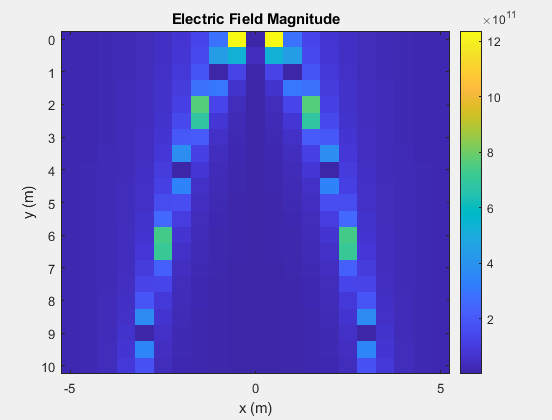
\includegraphics[scale=0.85]{figures/Figure_3.png}
  \caption{Electric Field Magnitude above the Ground Plate.}
\end{figure}

\nsection{Question 5}

\nsubsection{Problem Statement}
We want to calculate the induced electromotive force (EMF) in an elliptical loop under a time-varying magnetic field. The loop is defined by the equation:
\begin{equation}
  \frac{x^2}{a^2} + \frac{y^2}{b^2} = 1,
\end{equation}
and the magnetic field is given as:
\begin{equation}
  B(x, t) = e^{-x^2} \cos(\omega t).
\end{equation}

\nsubsection{Solution}

The induced EMF in the loop is determined using Faraday's Law:
\begin{equation}
\mathcal{E}mf = -\frac{d\Phi}{dt},
\end{equation}
where the magnetic flux \(\Phi\) is the integral of the magnetic field over the area of the ellipse:

\begin{align}
  \Phi(t) &= \int_{-a}^{a} \int_{-y}^{y} B(x, t) \, dy \, dx\\
          &= \int_{-a}^{a} \int_{-\sqrt{b^2\left(1 - \frac{x^2}{a^2}\right)}}^{\sqrt{b^2\left(1 - \frac{x^2}{a^2}\right)}} B(x,t) \, dy \, dx \\
          &= \int_{-a}^{a} \int_{-\sqrt{b^2\left(1 - \frac{x^2}{a^2}\right)}}^{\sqrt{b^2\left(1 - \frac{x^2}{a^2}\right)}}  e^{-x^2} \cos(\omega t) \, dy \, dx \\
\intertext{Since the magnetic field is only a function of \(x\), the integral over \(y\) can be simplified to:}
          &= \int_{-a}^{a} 2b \sqrt{1 - \frac{x^2}{a^2}} e^{-x^2} \cos(\omega t) \, dx
.\end{align}

The EMF is then calculated by taking the derivative of the magnetic flux with respect to time, and because the only time-dependent term is the cosine function, the derivative simplifies to, we consider the time derivative of the magnetic flux:

\begin{equation}
  \frac{\partial B}{\partial t} = -\omega e^{-x^2} \sin(\omega t).
\end{equation}
thus the EMF is given by:
\begin{equation}
  \mathcal{E}mf(t) = \omega \int_{-a}^{a} 2b \sqrt{1 - \frac{x^2}{a^2}} e^{-x^2} \sin(\omega t) \, dx.
\end{equation}

Considering the above expression, we can see that the EMF is a function of the semi-major axis \(a\), the semi-minor axis \(b\), and the frequency of the magnetic field \(\omega\). The magnitude of the induced EMF can be calculated by numerically integrating the above expression over the range \([-a, a]\) for various values of \(a\) and \(b\).

\nsubsection{MATLAB Implementation}

The calculation is implemented in MATLAB by numerically integrating the above expression over \([-a, a]\) for various values of \(a\) and \(b\). The following steps are performed:

\begin{enumerate}
    \item Define the parameters \(a\) and \(b\) to vary from 1 to 10 with a step of 0.5.
    \item Use a nested loop to compute the EMF for each combination of \(a\) and \(b\).
    \item define the EMF function as a function of \(x\) for each combination of \(a\) and \(b\).
    \item Integrate the function numerically using MATLAB's \texttt{integral} function.
    \item Plot the results in a 3D surface plot.
\end{enumerate}

\begin{minted}{python}
% Define parameters
a_vals = 1:0.5:10;  % Range of a
b_vals = 1:0.5:10;  % Range of b
omega = 1;          % Frequency of the magnetic field
t = pi/omega;     % Time period of the magnetic field

% Initialize matrix to store emf values
emf_vals = zeros(length(a_vals), length(b_vals));

% Loop over values of a and b
for i = 1:length(a_vals)
    for j = 1:length(b_vals)
        a = a_vals(i);
        b = b_vals(j);
        
        % Define the emf function
        emf_func = @(x) 2 * omega * b * sqrt(1 - (x.^2 / a^2)) .* exp(-x.^2) * sin(omega*t);
        
        % Compute emf using numerical integration
        emf_vals(i, j) = integral(emf_func, -a, a);
    end
end

% Plot the results in 3D
[A, B] = meshgrid(a_vals, b_vals);
figure;
surf(A, B, emf_vals');
xlabel('a');
ylabel('b');
zlabel('emf');
title('Magnitude of Induced emf vs a and b for Ellipse Path (t = pi/\omega)');
\end{minted}

\nsubsection{Results}

The magnitude of the induced EMF is plotted as a function of the semi-major axis \(a\) and the semi-minor axis \(b\) for an elliptical path at \(t = \frac{\pi}{\omega}\). The plot shows that the magnitude of the induced EMF increases with increasing values of \(a\) and \(b\), as expected.

\begin{figure}[ht]
  \centering
  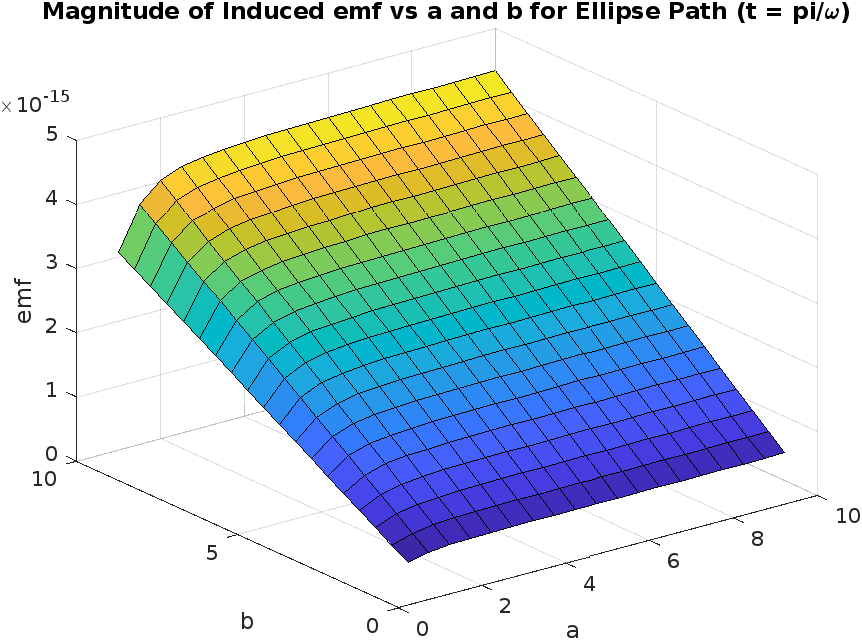
\includegraphics[scale=0.85]{figures/Figure_5.png}
  \caption{Magnitude of Induced EMF vs \(a\) and \(b\) for Elliptical Path at \(t = \frac{\pi}{\omega}\) with \(\omega = 1\).}
\end{figure}


\nsection{Question 6}

\nsubsection{Problem Statement}
For a certain structure, the magnetic field is given as follows:

\begin{table}[ht]
\centering
\renewcommand{\arraystretch}{2}
\begin{tabular}{|c|c|}
\hline
\textbf{Component} & \textbf{Expression} \\
\hline
$H_x$ & $\frac{j \beta m \pi}{k_c^2 a} A \sin\left(\frac{m \pi x}{a}\right) \cos\left(\frac{n \pi y}{b}\right) e^{-j \beta z}$ \\
\hline
$H_y$ & $\frac{-j \omega \mu m \pi}{k_c^2 a} A \sin\left(\frac{m \pi x}{a}\right) \cos\left(\frac{n \pi y}{b}\right) e^{-j \beta z}$ \\
\hline
$H_z$ & $A \cos\left(\frac{m \pi x}{a}\right) \cos\left(\frac{n \pi y}{b}\right) e^{-j \beta z}$ \\
\hline
$K_c$ & $\sqrt{\left(\frac{m \pi}{a}\right)^2 + \left(\frac{n \pi}{b}\right)^2}$ \\
\hline
$\beta$ & $\sqrt{k^2 - K_c^2}$ \\
\hline
$K$ & $\omega \sqrt{\mu \epsilon}$ \\
\hline
\end{tabular}
\caption{Magnetic field components and constants.}
\end{table}

It is required to plot the magnitude of \(E_x\) at different values of \(m\) and \(n\) (called different modes, which will be discussed next semester) versus \(x\) and \(y\) (contour plot). Let the frequency be \(1 \, \text{GHz}\), \(a = 1 \, \text{cm}\), \(b = 1 \, \text{cm}\), and \(A = 1\). Fill in the following table:

\begin{table}[ht]
\centering
\begin{tabular}{|c|c|c|c|}
\hline
$|E_x|$ & $m = 1$ & $m = 2$ & $m = 3$ \\
\hline
$n = 1$ &         &         &         \\
\hline
$n = 2$ &         &         &         \\
\hline
$n = 3$ &         &         &         \\
\hline
\end{tabular}
\caption{Table to fill with computed values of $|E_x|$ for different modes.}
\end{table}

\nsubsection{MATLAB Implementation}

The MATLAB implementation calculates and plots the magnitude of \(E_x\) for various modes (\(m, n\)) using the equations provided. The following steps are performed:

\begin{enumerate}
    \item Define parameters for the waveguide (\(a, b, \omega, \mu, \epsilon\)).
    \item Compute the constants \(K_c\), \(\beta\), and \(K\) for each mode (\(m, n\)).
    \item Calculate \(E_x\) over a 2D spatial grid of \(x\) and \(y\).
    \item Plot contour plots of \(|E_x|\) for each combination of \(m\) and \(n\).
\end{enumerate}

\begin{minted}{matlab}
% Constants
f = 1e9; % Frequency in Hz (1 GHz)
a = 1e-2; % Width of the waveguide in meters (1 cm)
b = 1e-2; % Height of the waveguide in meters (1 cm)
A = 1; % Amplitude
mu0 = 4 * pi * 1e-7; % Permeability of free space
epsilon0 = 8.854e-12; % Permittivity of free space
c = 3e8; % Speed of light in vacuum
omega = 2 * pi * f; % Angular frequency
k = omega / c; % Wave number in free space

% Spatial grid
x = linspace(0, a, 100); % x from 0 to a
y = linspace(0, b, 100); % y from 0 to b
[X, Y] = meshgrid(x, y);

% Modes to calculate
m_values = [1, 2, 3];
n_values = [1, 2, 3];

% Loop over modes and plot
figure;
for m = m_values
    for n = n_values
        % Calculate constants
        kc = sqrt((m * pi / a)^2 + (n * pi / b)^2); % Cutoff wave number
        beta = sqrt(k^2 - kc^2); % Propagation constant
        K = omega * sqrt(mu0 * epsilon0); % Wave number in medium

        % Calculate E_x
        Ex = -1j * beta / (kc^2) * A .* (m * pi / a) .* cos(m * pi * X / a) .* ...
            sin(n * pi * Y / b);

        % Magnitude of E_x
        Ex_magnitude = abs(Ex);

        % Plot contour
        subplot(length(m_values), length(n_values), (m-1)*length(n_values) + n);
        contourf(X, Y, Ex_magnitude, 20, 'LineColor', 'none');
        colorbar;
        colormap turbo; % Change colormap
        c = colorbar;
        c.Label.String = '|E_x| (Magnitude)';
        c.Label.FontSize = 10;
        title(['|E_x| for m = ' num2str(m) ', n = ' num2str(n)]);
        xlabel('x (m)', 'FontSize', 10);
        ylabel('y (m)', 'FontSize', 10);
    end
end

% Adjust figure layout
sgtitle('Magnitude of E_x for Different Modes', 'FontSize', 12);
\end{minted}

\nsubsection{Results}

The contour plots of \(|E_x|\) are generated for \(m = 1, 2, 3\) and \(n = 1, 2, 3\), showing the spatial variation of the electric field magnitude for different modes.

\begin{figure}[ht]
  \centering
  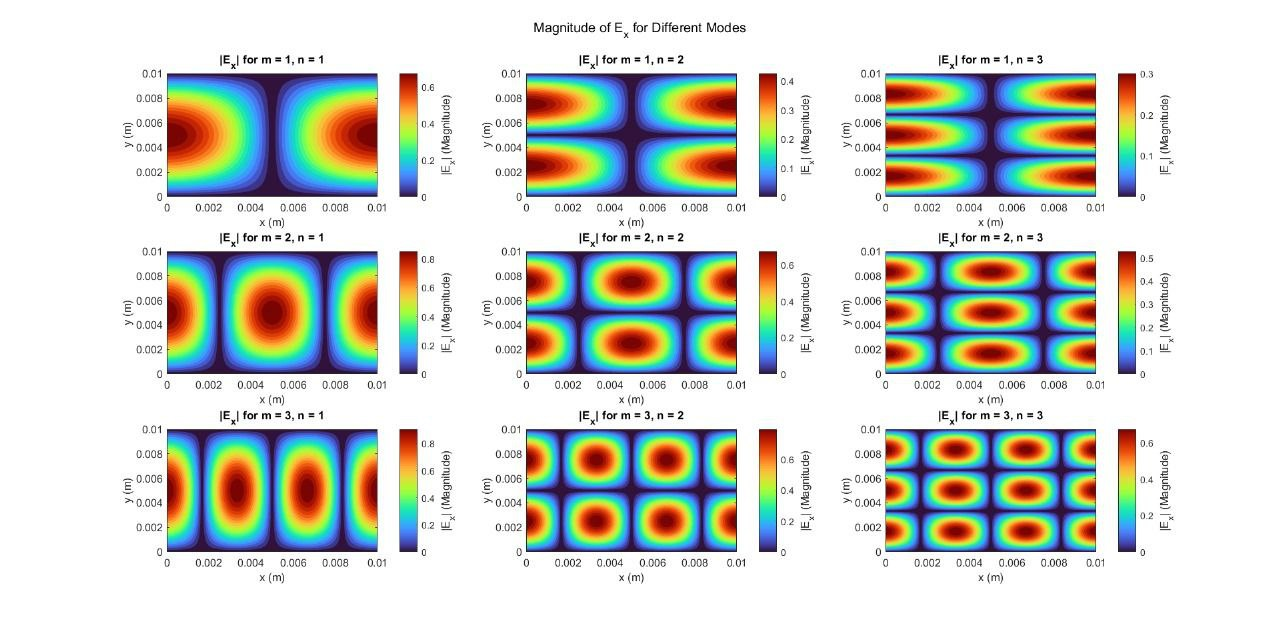
\includegraphics[scale=0.35]{figures/Figure_6.jpg}
  \caption{Contour plots of $|E_x|$ for various $m$ and $n$ modes.}
\end{figure}

\end{document}

